\section{Invereses and determinants}
\subsection{Inverse}
\definition{Inverse function}{
    Let $T:U\to V$ be bijective.
    The \textbf{inverse of} $T$ is the unique function $T^{-1}$ that satisfies
    \begin{align*}
        T^{-1}(T(x))= x,\\
        T(T^{-1}(y))=y
    \end{align*}
    for all $x\in U, y\in V$.\\
    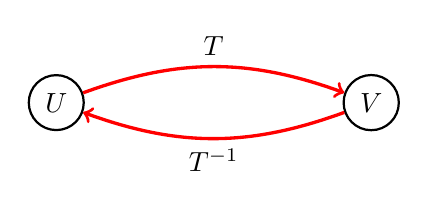
\begin{tikzpicture}
		\begin{scope}[every node/.style={circle,thick,draw}]
			\node (A) at (0,0) {$U$};
			\node (B) at (4,0) {$V$};
		\end{scope}
	
\begin{scope}[
	every edge/.style={draw=red,very thick}]
\path [->] (A) edge [bend left=20] node [above,midway]{$T$} (B);
\path [->] (B) edge [bend left=20]node [below,midway]{$T^{-1}$} (A);
\end{scope}
	\end{tikzpicture}
}
How do we know this inverse exists? We know that for each $y\in V$ there is exactly one
$x\in U$ that satisifes $T(x)=y$, so we can set $T^{-1}(y)$ to be this particular value of $x$ for each y.
This definition of the inverse sounds tautological, so let us apply this to linear transformations.
\proposition{
    Let $T:\reals^n\to\reals^n$ be a bijective linear transformation.
    Then $T^{-1}$ is a linear transformation.
}
\begin{proof}
    We want to show that for any $\vec{y}_1,\vec{y}_2\in\reals^n$, $c\in \reals$,
    $T^{-1}(\vec{y}_1+\vec{y}_2)=T^{-1}(\vec{y}_1)+T^{-1}(\vec{y}_2)$ and $T^{-1}(c\vec{y}_1)=cT^{-1}(\vec{y}_1)$.

    The trick to solving this is to use the definition for inverses and switch back and forth with $T$ and $T^{-1}$, and apply linearity of $T$.
    \begin{align*}
        T^{-1}(\vec{y}_1)+T^{-1}(\vec{y}_2) &= T^{-1}(T(T^{-1}(\vec{y}_1)+T^{-1}(\vec{y}_2)))\\
        &=T^{-1}(T(T^{-1}(\vec{y}_1))+T(T^{-1}(\vec{y}_2))) \textrm{ (as $T$ is linear)}\\
        &=T^{-1}(\vec{y}_1+\vec{y}_2).
    \end{align*}
    For scaling,\begin{align*}
        cT^{-1}(\vec{y}_1) &= T^{-1}(T(cT^{-1}(\vec{y_1})))\\
        &=T^{-1}(c(T(T^{-1}(\vec{y_1}))))\\
        &=T^{-1}(c\vec{y}_1).
    \end{align*}
\end{proof}
This means that the inverse of $T$ has a matrix representation.
If we write $T(\vec{x})=A\vec{x}$ for some matrix $A$,
then there is some matrix $B$ such that $AB=BA=I_n$.
\definition{Matrix Inverses}{
    Let $A\in M_{m\times n}(\reals)$. If there exists $X\in M_{n\times m}(\reals)$ such that
    \[
    XA=I_n,
    \]
    we call $X$ the \textbf{left inverse} of $A$.
    Similarly, if there exists $Y\in M_{n\times m}(\reals)$ such that
    \[
        AY=I_m,
    \]
    we call $Y$ the \textbf{right inverse} of $A$.
    If both the left and right inverses exist and are equal, then we say that $A$ is \textbf{invertible}, and denote $X=Y$ the \textbf{inverse} of $A$, written as $A^{-1}$.
}
\begin{remark}
    If $A$ has a left and right inverse, then the left and right inverses are equal. Indeed, we have for a left inverse $X$ and a right inverse $Y$ of $A$,\[
    X= X(I_m)= X(AY) = (XA)Y = (I_n)Y = Y.
    \]
\end{remark}
As we have already seen, only bijective linear transformations have inverses, so that means we have more to add to That One Theorem. We also see that being invertible implies having a left and right inverse, so might expect that having a left or right inverse corresponds to the columns being linearly independent or span $\reals^m$. 
\example{
    $A\in M_{m\times n}(\reals)$ having a left/right inverse indeed corresponds to the conditions that the columns are linearly independent and the columns span $\reals^m$. Figure out which conditions correspond to each other.
}
There are two ways to think about this problem: one way is directly translate left and right inverses to the corresponding statements of the column vectors; the other way is to think of them in linear transformations and find out which one is surjective/injective. I will outline both methods.

\textbf{Method 1:} 
Without knowing where to go, let us suppose we want to prove $A$ has linearly independent columns and see which extra hypothesis we need. Suppose \[
    A\vec{x}=\vec{0}.
\]
We want to show $\vec{x} = \vec{0}$. This means we want to cancel the $A$ on the left, so we want to use the left inverse $X$. \[
\vec{x}=XA\vec{x} = X\vec{0} = \vec{0}.
\] 
So this means having a left inverse corresponds to linear independence.
Now to prove the columns of $A$ span $\reals^m$, we try to solve \[
A\vec{x}=\vec{b}
\] for any $\vec{b}\in\reals^m$.
To produce a solution $\vec{x}$ that can cancel $A$ from the right, we will need the right inverse $Y$, and set $\vec{x}=Y\vec{b}$, then
\[
A\vec{x}=AY\vec{b}=\vec{b}.
\]

\textbf{Method 2:}
We translate the problem into a linear transformation $T:\reals^n\to\reals^m$ being injective (linear independence) and surjective (span $\reals^m$).
Why does a left inverse imply injectivity? Let us suppose $T(\vec{x})=T(\vec{y})$, then the left inverse can immediately cancel out the $T$ from the left and give us $\vec{x}=\vec{y}$.

For surjectivity, let us break down the columns of the right inverse $Y=\begin{bmatrix}
    \vec{y}_1 & \ldots &\vec{y}_m
\end{bmatrix}$.
Then by the property of matrix multipication, we can consider each column to see \[
A\vec{y}_j = \vec{e}_j.
\]
Since the basis vectors can build anything in $\reals^m$, we can just use the corresponding linear combination of the $\vec{y}_j$'s to build anything in $\reals^m$.
This means we have three extra equivalences for a matrix being invertible.

\theorem{This/That One}{
    Let $A=[\vec{v}_1\ldots \vec{v}_n]\in M_{n\times n}(\reals)$, and $T:\reals^n\to\reals^n$ be the unique linear transformation satisfying $T(\vec{x})=A\vec{x}$ for all $\vec{x}\in\reals^n$.
	Then the following are equivalent.
	\begin{enumerate}
		\item $\{\vec{v}_1,\ldots,\vec{v}_n\}$ form a basis.
		\\ $\vdots$
	\end{enumerate}
	
	\begin{thatonethmlist}
		\item $A$ is invertible.
		\item $A$ as a left inverse.
		\item $A$ has a right inverse.
	\end{thatonethmlist}
}
\subsection{Isomorphisms}
\definition{Isomorphism}{
	Let $T:U\to V$ be a bijective linear transformation. We call $T$ an \textbf{isomorphism} and the vector spaces $U$ and $V$ are \textbf{isomorphic}. We denote this $U\simeq V$.
}
Recall many sections ago, we said that many types of vector spaces are very similar to $\reals^n$. Now that we have defined isomorphic vector spaces, we have a concrete statement of what it means to be similar.
\theorem{Finite dimensional real vector spaces $\simeq \reals^n$ }{
Let $V$ be a finite dimensional real vector spaces. Then $V\simeq \reals^n$ for some $n\in\mathbb{N}$.
}
\begin{proof}
	Since $V$ is finite dimensional, let $\{v_1,...,v_k\}$ be a basis for $V$.
	We just need to construct an isomorphism from $\reals^n \to V$. What is an easy way to define this? We just need to define where each of the standard basis vectors $\vec{e}_j$ goes. This gives us a very natural choice to guess that the isomorphism $T:\reals^k\to V$ defined by \[
		T(\vec{e}_j)=v_j,	
	\]
	or equivalently \[
	T(\vec{x})=x_1v_1+x_2v_2+\ldots+x_kv_k
	\]
	is bijective. This is indeed bijective, which you have confirmed in a previous exercise.	
\end{proof}
\corollary{
	Let $V$ be finite dimensional. Then every basis of $V$ has the same number of vectors.
}
\begin{proof}
	Let $\{v_1,\ldots,v_k\}$ and ${w_1,\ldots, w_l}$ be two bases for $V$. Then by the construction in the previous theorem, we have $V\simeq \reals^k$ and $V\simeq \reals^l$. So $\reals^k\simeq \reals^l$ and thus $k=l$.
\end{proof}
\subsection{Determinants}
We now move towards the last equivalence for That One Theorem. Recall in the intuition behind the \href{thm:2.48}{Matrix Represnetation of Linear Transformations}, we constructed a grid and showed that a linear transformation is a change in the coordinate system.\\
\begin{figure}[h]
	\begin{subfigure}[l]{0.4\textwidth}
		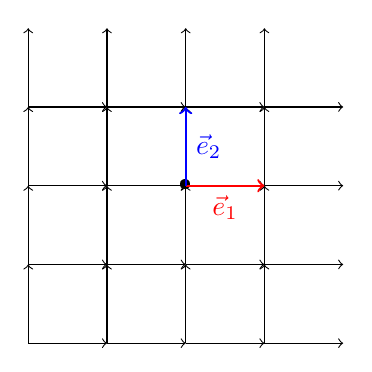
\begin{tikzpicture}
			\draw (0,0) node{\textbullet};
			\foreach \i in {-2,...,1}{
				\foreach \j in {-2,...,1}{
					\draw [->,thin] (\i,\j)--(\i+1,\j);
					
					\draw [->,thin] (\i,\j)--(\i,\j+1);
				}
			}
			\draw [->,color=red,thick] (0,0)--(1,0) node[midway, below]{$\vec{e}_1$} ;
			\draw [->,color=blue,thick] (0,0)--(0,1) node [right,midway]{$\vec{e}_2$};
			\end{tikzpicture}
			\caption{Original grid}
	\end{subfigure}
	\begin{subfigure}[r]{0.6\textwidth}
		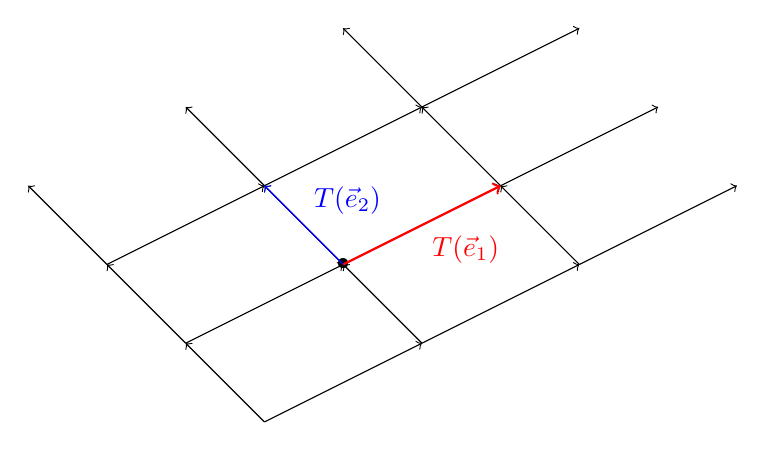
\begin{tikzpicture}
			\draw (0,0) node{\textbullet};
			\foreach \i in {-1,...,1}{
				\foreach \j in {-1,...,1}{
					\draw [->,thin] (\i*2-\j,\j+\i)--(\i*2-\j+2,\i+\j+1);
					
					\draw [->,thin] (\i*2-\j,\j+\i)--(\i*2-\j-1,\i+\j+1);
				}
			}
			\draw [->,color=red,thick] (0,0)--(2,1) node[midway, below right ]{$T(\vec{e}_1)$} ;
			\draw [->,color=blue] (0,0)--(-1,1) node [above right ,midway,thick]{$T(\vec{e}_2)$};
			\end{tikzpicture}
			\caption{Transformed grid}
	\end{subfigure}
\end{figure}
The original grid squares become grid `parallelograms'. Indeed, if you extend to three dimensions, you can get grid `parallelepipeds'.
To say that the transformation is surjective means that the transformed unit square/cubes have non-zero area/volume and can thus tessellate.



\begin{figure}[h]
	\begin{subfigure}[l]{0.4\textwidth}
		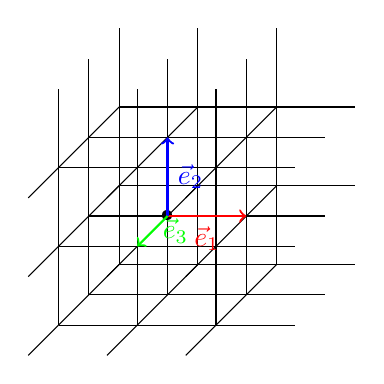
\begin{tikzpicture}
			\draw (0,0) node{\textbullet};
			\foreach \i in {-1,...,1}{
				\foreach \j in {-1,...,1}{
                    \foreach \k in {-1,...,1}{

					\draw [-,thin] (\i,\j,\k)--(\i+1,\j,\k);
					
					\draw [-,thin] (\i,\j,\k)--(\i,\j+1,\k);
					\draw [-,thin] (\i,\j,\k)--(\i,\j,\k+1);
                    }
				}
			}
			\draw [->,color=red,thick] (0,0,0)--(1,0,0) node[midway, below]{$\vec{e}_1$} ;
			\draw [->,color=blue,thick] (0,0,0)--(0,1,0) node [right,midway]{$\vec{e}_2$};
            \draw [->,color=green,thick] (0,0,0)--(0,0,1) node [right,midway]{$\vec{e}_3$};
			\end{tikzpicture}
			\caption{Original grid}
	\end{subfigure}
	\begin{subfigure}[r]{0.6\textwidth}
		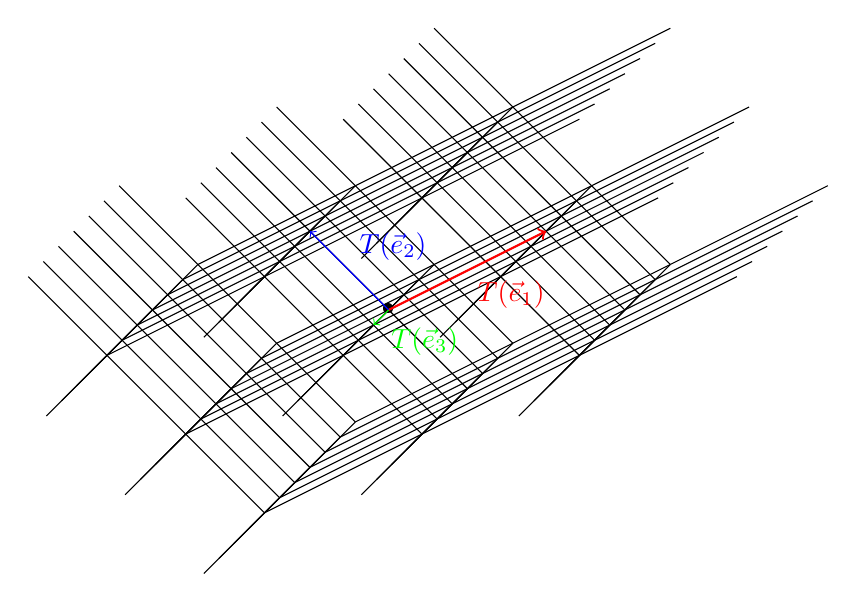
\begin{tikzpicture}
			\draw (0,0) node{\textbullet};
			\foreach \i in {-1,...,1}{
				\foreach \j in {-1,...,1}{
                    \foreach \k in {-3,...,3}{

					\draw [-,thin] (\i*2-\j,\j+\i,0.5*\k)--(\i*2-\j+2,\i+\j+1,0.5*\k);
					
					\draw [-,thin] (\i*2-\j,\j+\i,0.5*\k)--(\i*2-\j-1,\i+\j+1,0.5*\k);
					\draw [-,thin] (\i*2-\j,\j+\i,0.5*\k)--(\i*2-\j,\i+\j,0.5*\k+2);
                    }
				}
			}
			\draw [->,color=red,thick] (0,0)--(2,1) node[midway, below right ]{$T(\vec{e}_1)$} ;
			\draw [->,color=blue] (0,0)--(-1,1) node [above right ,midway,thick]{$T(\vec{e}_2)$};
			\draw [->,color=green] (0,0,0)--(0,0,0.5) node [below right,midway,thick]{$T(\vec{e}_3)$};
			\end{tikzpicture}
			\caption{Transformed grid}
	\end{subfigure}
    \caption{I tried my best, please use a bit of imagination}
\end{figure}

